% Autor: Leonhard Segger, Alexander Neuwirth
% Datum: 2017-10-21
\documentclass[
	% Papierformat
	a4paper,
	% Schriftgröße (beliebige Größen mit „fontsize=Xpt“)
	12pt,
	% Schreibt die Papiergröße korrekt ins Ausgabedokument
	pagesize,
	% Sprache für z.B. Babel
	ngerman
]{scrartcl}

% Achtung: Die Reihenfolge der Pakete kann (leider) wichtig sein!
% Insbesondere sollten (so wie hier) babel, fontenc und inputenc (in dieser
% Reihenfolge) als Erstes und hyperref und cleveref (Reihenfolge auch hier
% beachten) als Letztes geladen werden!

% Silbentrennung etc.; Sprache wird durch Option bei \documentclass festgelegt
\usepackage{babel}
% Verwendung der Zeichentabelle T1 (Sonderzeichen etc.)
\usepackage[T1]{fontenc}
% Legt die Zeichenkodierung der Eingabedatei fest, z.B. UTF-8
\usepackage[utf8]{inputenc}
% Schriftart
\usepackage{lmodern}
% Zusätzliche Sonderzeichen
\usepackage{textcomp}

% Mathepaket (intlimits: Grenzen über/unter Integralzeichen)
\usepackage[intlimits]{amsmath}
% Ermöglicht die Nutzung von \SI{Zahl}{Einheit} u.a.
\usepackage{siunitx}
% Zum flexiblen Einbinden von Grafiken (\includegraphics)
\usepackage{graphicx}
% Abbildungen im Fließtext
\usepackage{wrapfig}
% Abbildungen nebeneinander (subfigure, subtable)
\usepackage{subcaption}
% Funktionen für Anführungszeichen
\usepackage{csquotes}
% Zitieren, Bibliographie
\usepackage{biblatex}

% Verlinkt Textstellen im PDF-Dokument
\usepackage[unicode]{hyperref}
% "Schlaue" Referenzen (nach hyperref laden!)
\usepackage{cleveref}
% Zur Darstellung von Webadressen
\usepackage{url}

% siunitx: Deutsche Ausgabe, Messfehler getrennt mit ± ausgeben
\sisetup{
	locale=DE,
	separate-uncertainty
}

\begin{document}
	\begin{titlepage}
		\centering
		{\scshape\LARGE Versuchsbericht zu \par}
		\vspace{1cm}
		{\scshape\huge S1 -- Was ist Experimentieren?\par}
		\vspace{2.5cm}
		{\LARGE Gruppe 6Mi \par}
		\vspace{0.5cm}
		
		{\large Alexander Neuwirth (E-Mail: a\_neuw01@wwu.de) \par}
		{\large Leonhard Segger (E-Mail: l\_segg03@uni-muenster.de) \par}
		\vfill
		
		durchgeführt am 18.10.2017\par
		betreut von\par
		{\large Dr. Anke \textsc{(Beck-)Schmidt}} %Ich hoffe, das ist ok stumpf die zu nehmen.
		
		\vfill
		
		{\large \today\par}
	\end{titlepage}
	\tableofcontents
	
	\newpage
	\section{Beantworten Sie diese Fragen:}
	
	\subsection{Was ist mit "Messgröße" gemeint?}
	Eine Messgröße ist eine mithilfe eines Messverfahrens an einer physikalischen Gegebenheit ermittelter Zahlenwert mit Maßeinheit. Der Messwert wird für gewöhnlich von der Anzeige eines Messgerätes abgelesen oder durch einen Computer automatisiert erfasst. Er ist abhängig von Messunsicherheiten oder der nur eingeschränkt kontrollierbaren Versuchsumgebung. Deshalb ist es mit Messgrößen auch immer nur möglich den \textit{wahren Wert} als mit einer bestimmten Wahrscheinlichkeit in einem gegebenen Intervall liegend zu bestimmen. Beispiele für Messgrößen sind Lägen, Massen, Volumina oder Kräfte. Wie am Beispiel der Volumina erkennbar, muss die Messgröße nicht unmittelbar erfassbar sein, sondern kann sich auch aus anderen Messgrößen ergeben (hier aus der Länge).
	
	\subsection{Warum führt man in der Naturwissenschaft Experimente durch?}
	In der Mathematik sind einige geschickt gewählte Prämissen ausreichend, um alles, was man untersuchen möchte, logisch herzuleiten. In den Naturwissenschaften kennen wir diese natürlichen Prämissen nicht und sind daher darauf angewiesen, eine \enquote{Top-Down-Perspektive} anzunehmen. Wir können nur die Effekte der Prämissen beobachten und müssen daraus dann Rückschlüsse auf die grundlegenden Konzepte finden. Ein Beobachten dieser Effekte nennt man dann \enquote{Experiment} und ist aus der Naturwissenschaft nicht wegzudenken. Außerdem wäre man ohne tatsächliche Messungen nicht in der Lage die aufgestellten Theorien zu überprüfen und zu quantifizieren.
	
	\subsection{Warum kann der “wahre Wert” einer Messgröße niemals bestimmt werden?}
	Einerseits hat jedes Messgerät eine Unsicherheit und auch eine große Anzahl an Messungen schränkt das Intervall, in dem der \enquote{wahre Wert} der Messgröße mit hoher Wahrscheinlichkeit liegt, nur ein. Eine Messung des wahren Wertes würde ein unendlich genaues Messgerät oder eine unendliche Zahl an Messungen voraussetzen. Dies wird sich aus offensichtlichen Gründen niemals realisieren lassen. Außerdem würde eine exakte Messung auch eine exakte Kontrolle der Randbedingungen des Experiments benötigen. Wie unrealistisch dies ist, lässt sich daran erkennen, dass beispielsweise der gravitationelle Einfluss eines Staubkorns im Nachbargebäude des Raumes, in dem das Experiment durchgeführt wird, in die Rechnung einbezogen werden müsste.
	
	\section{Durchgeführte Versuche}
	%TODO: Skizzen?
	\subsection{Versuch 1: Leerlaufspannung einer Batterie}
	
	\subsubsection{Fragestellung}
	Welche Spannung hat die vorliegende 9-Volt-Batterie?
	\subsubsection{Vorwissen}
	Batterien haben unmittelbar nach der Herstellung eine höhere Spannung als angegeben, da sie sich mit zunehmender Aufbewahrungsdauer selbst entladen. Die aufgedruckte Spannung soll bis zum angegebenen Datum (in diesem Fall Februar 2017) vorhanden sein. Demnach ist es unwahrscheinlich, dass die Batterie noch eine höhere Spannung als 9V hat. Da wir keine Informationen über ihre bisherige Nutzung haben, lassen sich allerdings keine weiteren Schlüsse über den Zustand ihrer Ladung ziehen. Also ist ihre Leerlaufspannung auf 0-9 Volt einzuschätzen, ohne dass man nähere Angaben dazu machen könnte, welche Spannungsbereiche wahrscheinlicher als andere sind. Demnach ergibt sich eine rechteckige WDF, wie sie im Laborbuch (Seite 1) zu sehen ist. 
	\subsubsection{Darstellung der Messwerte}
	Es wurde mit einem Multimeter gemessen. Dabei wurde der Messbereich verkleinert, bis der Messwert darin lag. Dies war im Bereich 2V bis 20V der Fall.  Da der angezeigte Wert auf der Digitalanzeige bei längerer Messung leicht schwankte haben wir versucht den Wert aufzunehmen, der sich kurz nach Beginn der Messung einstellte, um nicht durch den endlichen Innenwiederstand (und den dadurch entstehenden Stromfluss) des Multimeters den Ladungsstand der Batterie zu beeinflussen. %EDIT: ergänzt

	\begin{tabular}{| c | c |}
		\hline
		Messung & Leerlaufspannung $U_0$ / \si{V}\\ \hline
		1 & 5,67\\
		2 & 5,61\\ \hline
	\end{tabular}
	\subsubsection{Unsicherheitsbetrachtung}
	Der Hersteller der Multimeter gibt eine Messtoleranz von ±0,5\% des abgelesenen Wertes für Gleichspannungsmessungen in den Messbereichen 2 V und 20 V an. Die ist eine Typ B Unsicherheit mit rechteckiger WDF. Außerdem lässt sich die Spannung nur bis auf zwei Nachkommastellen ablesen, wodurch eine zusätzliche Ungenauigkeit von $\pm 0,005\si{V}$ entsteht. Dies ist ebenfalls eine Typ B Unsicherheit mit rechteckiger WDF. Insgesamt ergibt sich: \\
	$u_1= \frac{0,01}{2\sqrt{3}} \si{V} \approx 0,0029 \si{V}$ \\
	$u_2= \frac{2 \cdot 0,005 \cdot \text{Messwert}}{2 \sqrt{3}}$ \\ %kp ob das schön ist
	Messung 1: Unsicherheit: $\pm \sqrt{(\frac{0,01 \cdot 5,67}{2 \sqrt{3}})^2 + 0,0029^2} \si{V} \approx \pm 0,075 \si{V}$ \\
	Messung 2: Unsicherheit: $\pm \sqrt{(\frac{0,01 \cdot 5,61}{2 \sqrt{3}})^2 + 0,0029^2} \si{V} \approx \pm 0,074 \si{V}$ 
	
	\subsubsection{Ergebnis}
	\begin{tabular}{| c | c |}
		\hline
	Messung & Leerlaufspannung $U_0$ / \si{V}\\ \hline
	1 & \SI{5,67 +- 0,075}{\V}\\ %\hline
	2 & \SI{5,61 +- 0,074}{\V}\\ \hline
	\end{tabular} \\
	Mittelwert $\overline{U}_0= 5,64 \si{V}$ \\
	Unsicherheit Mittelwert: $u_{\text{M},\leq10}=t_{68}(3)\sqrt{\frac{\sum_{i=1}^{n} (x_i-\overline{x})^2}{n(n-1)}}=0,036 \si{V}$ \newline
	kombinierte Unsicherheit: $\pm \sqrt{(u_\text{M})^2 + 0,0029^2} \si{V} \approx \pm 0.036 \si{V}$ 
	%Unsicherheit Mittelwert $u_{\overline{U}} = $
	%TODO: Wie mach ich das, weil ist nicht Gauß, studentsche t- verteilung bissl überzogen oder?
	\subsubsection{Schlussfolgerung}
	Die Leerlaufspannung liegt höchstwahrscheinlich bei $U_0=\SI{5,64 \pm 0.036}{V}$. Die lässt darauf schließen, da das \enquote{Haltbarkeitsdatum} der Batterie noch nicht so lange überschritten ist, dass eine derartige Entladung zu erwarten wäre, dass die Batterie bereits benutzt wurde. %TODO: Hier Unsicherheit angeben
	
	\newpage
	\subsection{Versuch 2: Länge eines Stiftes}
	
	\subsubsection{Fragestellung}
	Wie lang ist der vorliegende Stift?
	\subsubsection{Vorwissen}
	Eine grobe Abschätzung mit dem Auge ergibt ca. 14\si{cm}. Hierfür haben wir uns den Messbereich eines Geo-Dreiecks vorgestellt und dies mit dem Stift verglichen.
	\subsubsection{Darstellung der Messwerte}
	Ein Maßband wurde von einer Person an das eine Ende des Stiftes gehalten, während die andere Person am anderen Ende die Skala ablas.

	\begin{tabular}{| c | c |}
		\hline
		Messung Nr. & Länge l  / \si{cm}\\ \hline
		1 & 16,7\\
		2 & 16,7\\ \hline
	\end{tabular}
	\subsubsection{Unsicherheitsbetrachtung}
	Das Lineal lässt sich ungefähr mit einer Genauigkeit von $\pm 0,1 \si{cm}$ ablesen. Dies ist eine Typ B Unsicherheit mit dreieckiger WDF.
	$u=\frac{0,2}{2 \sqrt{6}} \si{cm}=0,04 \si{cm}$
	\subsubsection{Ergebnis}
	\begin{tabular}{| c | c |}
		\hline
		Messung Nr. & Länge l  / \si{cm}\\ \hline
		1 & \SI{16,7 \pm 0,04}{cm}\\
		2 & \SI{16,7 \pm 0,04}{cm}\\ \hline
	\end{tabular}
	\subsubsection{Schlussfolgerung}
	Die Länge des Stiftes kann als \SI{16,7 \pm 0,04}{cm} angenommen werden. Daraus lässt sich folgern, dass die Abschätzung mit dem Auge für eine grobe Einschätzung der Länge eines Stiftes ausreicht. Eine auf wenige Millimeter genaue Angabe der Länge setzt jedoch eine tatsächliche Messung voraus.
	\newpage
	\subsection{Versuch 3: Kugeln auf der schiefen Bahn}
	\subsubsection{Fragestellung}
	Rollt eine Metallkugel die schiefe Schiene schneller herunter als eine Holzkugel?
	\subsubsection{Vorwissen}
	Die bisher akzeptierte Hypothese ist, dass die schwerere Kugel, also die metallene, unter dem Einfluss der Reibung schneller rollt. Beim vertikalen Falle erwarten wir bei einer Messung, die nicht im Vakuum stattfindet, dass eine Holzkugel langsamer fällt als eine Metallkugel, da die Oberflächenstruktur der Holzkugel eine größere Bremswirkung durch den Luftwiderstand verursacht. Dies lässt sich auf ein Rollen mit dem Winkel $\alpha$ zur Horizontalen übertragen. Aus der Fallbeschleunigung ergibt sich: 
	$ma=mg \sin \alpha$.
	Da sich hier die Masse eliminiert, hat diese keinen Einfluss auf die Fallbeschleunigung. Wenn man lediglich das Trägheitsmoment betrachtet, würde man sogar ein langsameres Rollen der Metallkugel erwarten, da sie ein höheres Trägheitsmoment hat und somit langsamer beschleunigt wird.
	Wir messen so häufig, bis sich der laufende Mittelwert der Zeit, die die Kugel bis zum Ende der Schiene benötigt, nicht mehr wesentlich ändert.
	\subsubsection{Darstellung der Messwerte}
	
	\begin{tabular}{| c | c | c | c | c |} \hline
		Messung Nr. & Holz  / \si{s} & Metall  / \si{s} & HM  / \si{s} & MM  / \si{s}\\ \hline
		1 & 1,87&1,72&1,87&1,72\\
		2 & 1,84&1,62&1,86&1,67\\
		3 & 1,88&1,65&1,86&1,66\\
		4 & 1,75&1,72&1,84&1,68\\
		5 & 1,85&1,59&1,84&1,66\\
		6 & 1,90&1,69&1,85&1,65\\
		\hline
	\end{tabular}
	\newline
	HM (MM) ist hierbei der Laufende Mittelwert der Holzkugel (Metallkugel). \newline
	Standardunsicherheiten des Mittelwertes: \newline
	Holzkugel: $u_\text{HM}=t_{68}(3)\sqrt{\frac{\sum_{i=1}^{n} (x_i-\overline{x})^2}{n(n-1)}}=0,128 \si{s}$ \newline
	Metallkugel: $u_\text{MM}=0,144\si{s}$
	
	\begin{figure}[htb]
	  \centering
	    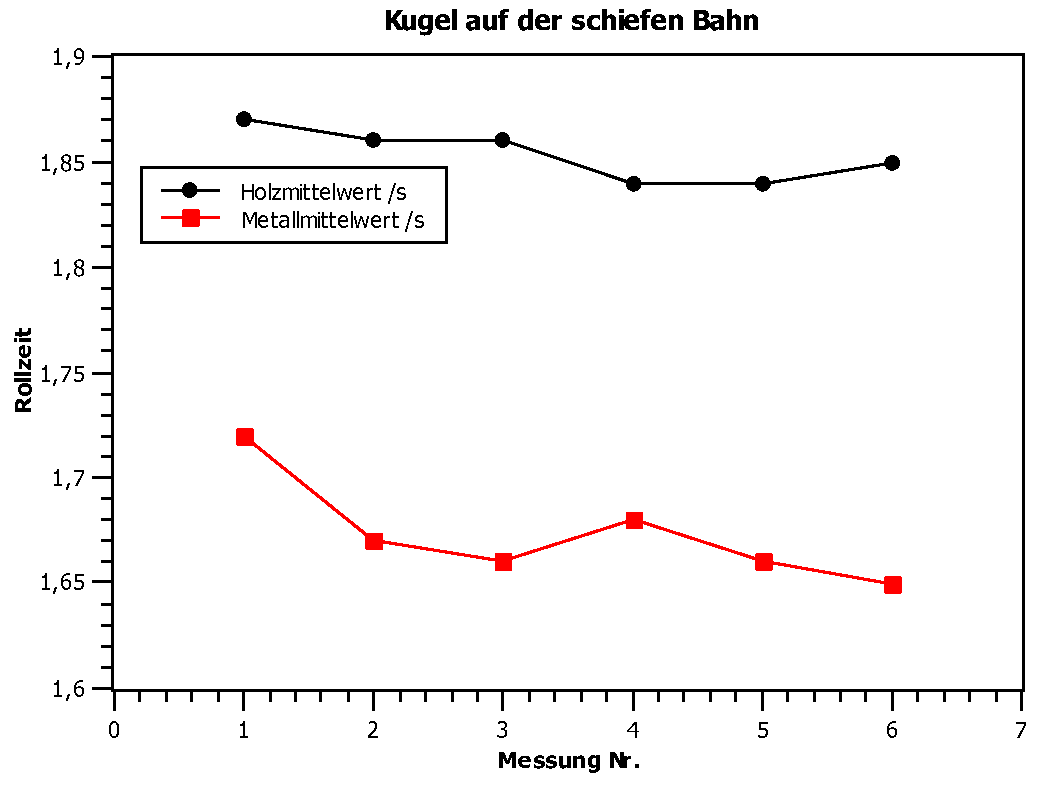
\includegraphics[width=0.6\textwidth]{Kugel_auf_schiefer_Bahn} % Keine Angabe der Dateiendung nötig, TeX durchsucht den Ordner, in dem dieser Quelltext liegt
	  \caption{Darstellung der laufenden Mittelwerte}
	\end{figure}
	\subsubsection{Unsicherheitsbetrachtung}
	Die menschliche Wahrnehmung limitiert die Genauigkeit der Zeitmessung mit einer Stoppuhr. Dies in einen Zahlenwert zu fassen würde einen separaten Vergleich von dieser Messmethode zu einer automatisierten (z.B. mit einer Lichtschranke) voraussetzen. Die Unsicherheit, die durch die Limitierung des Digitaldisplays auf zwei Nachkommastellen entsteht, dürfte demgegenüber zu vernachlässigen sein.
	\subsubsection{Ergebnis}
	Die Metallkugel rollt signifikant (Abweichung größer als Standardunsicherheit) schneller auf der Rinne.
	\subsubsection{Schlussfolgerung}
	Um die Hypothese legitimerweise in Frage zu stellen, müsste die Holzkugel im Mittel schneller die Bahn hinunterrollen als die Metallkugel und die Abweichung müsste größer sein als die Standardunsicherheit. Die erste Bedingung ist bereits nicht erfüllt, daher konnten wir die Hypothese nicht falsifizieren und sie kann beibehalten werden. Unsere Vorannahme, dass der Einfluss des Trägheitsmoments auf die Zeit, die die Kugel benötigt, um die schiefe Bahn hinunter zu rollen, gegenüber dem Reibungswiederstand verschwindet, wird also durch die Ergebnisse unterstützt.
	
	
\end{document}
